\documentclass[a4paper,12pt]{article}
\usepackage[left=2cm, right=2cm, top=2cm]{geometry}
\usepackage{graphicx} 
\usepackage[export]{adjustbox}
\usepackage{titlepic}
\usepackage{amssymb}
\usepackage{titling}
\usepackage[utf8]{inputenc}
\usepackage{listings}
\usepackage{color}
\usepackage[T1]{fontenc}
%\usepackage{fontspec}
\usepackage[%  
colorlinks=true,
pdfborder={0 0 0},
linkcolor=black
]{hyperref}
\usepackage[utf8]{inputenc}
\usepackage{wrapfig}
\usepackage{helvet}
\usepackage{fourier} 
\usepackage{array}
\usepackage{makecell}
\usepackage{subfig}
\usepackage[square,sort,comma,numbers]{natbib}
\usepackage{gensymb}
\usepackage{ragged2e}
\usepackage{placeins}
\bibliographystyle{IEEEtran}
\usepackage{float}
\setlength{\belowcaptionskip}{-15pt}
\renewcommand{\familydefault}{\sfdefault}
\newcommand{\squeezeup}{\vspace{-2.5mm}}
\definecolor{codegreen}{rgb}{0,0.6,0}
\definecolor{codegray}{rgb}{0.5,0.5,0.5}
\definecolor{codepurple}{rgb}{0.58,0,0.82}
\definecolor{backcolour}{rgb}{0.95,0.95,0.92}

\renewcommand\theadalign{bc}
\renewcommand\theadfont{\bfseries}
\renewcommand\theadgape{\Gape[4pt]}
\renewcommand\cellgape{\Gape[4pt]}

\usepackage{fancyhdr,lipsum}
\pagestyle{fancy}
\fancyhf{}% Clear header/footer

\usepackage{hyperref}
\hypersetup{
    colorlinks,
    %citecolor=gray,
    citecolor=black,
    filecolor=black,
    linkcolor=black,
    urlcolor=black,
    linktoc=all
}

\lstdefinestyle{mystyle}{
    backgroundcolor=\color{backcolour},   
    commentstyle=\color{codegreen},
    keywordstyle=\color{blue},
    numberstyle=\tiny\color{codegray},
    stringstyle=\color{codepurple},
    basicstyle=\tiny,
    breakatwhitespace=false,         
    breaklines=true,                 
    captionpos=b,                    
    keepspaces=true,                 
    numbers=left,                    
    numbersep=5pt,                  
    showspaces=false,                
    showstringspaces=false,
    showtabs=false,                  
    tabsize=2
}


\chead{%
  \ifcase\value{page}
  % empty test for page = 0
  \or Alexander Bolton% page=1
  \or Alexander Bolton% page = 2
  \or Alexander Bolton% page = 3
  \or Alexander Bolton% page = 4
  \or Alexander Bolton% page = 5
  \or Sam Wilcock% page = 6
  \or Sam Wilcock% page = 7
  \or Sam Wilcock% page = 8
  \or Sam Wilcock% page = 9
  \or Sam Wilcock% page = 10
  \or John Jakobsen% page = 11
  \or John Jakobsen% page = 12
  \or John Jakobsen% page = 13
  \or Alexander Bolton - Sam Wilcock - John Jakobsen% page = 14
  \or Alexander Bolton - John Jakobsen% page = 15
  \or % page = 16
  \or % page = 14
  \else
  % Empty chead here! Lovely cheddar
  \fi
}

\cfoot{\thepage}

\lstset{style=mystyle}

\pretitle{%
  \begin{center}
  \LARGE
\includegraphics[width=0.5\textwidth, right]{UniLogo.png}\\[\bigskipamount]

\hspace{15cm}

\hspace{27cm}

\hspace{27cm}

\hspace{10cm}
}
\posttitle{\end{center}}	

\begin{document}
\title{\\ \textbf{ELEC5620M \\ Mini Project \\ \- \\ DE1-SoC Pong }}
\author{Alexander Bolton - 200938078 \\ Sam Wilcock - 201285260\\ John Jakobsen - 201291841}
\date{May 2019}
\maketitle
\thispagestyle{empty}
\begin{center}

\end{center}
\vfill
\begin{center}
The University of Leeds \\  School of Electronic and Electrical Engineering
\end{center}

\newpage

\tableofcontents
\thispagestyle{empty}

\newpage 
\pagenumbering{arabic}
\section{Introduction}
\begin{flushleft}
This report will discuss the group project for the Embedded Microprocessor System Design module. The groups members were Alexander Bolton, Sam Wilcock, and John Jakobsen. The projects aim was to create a game of Pong on the DE1-SoC's microprocessor unit (MPU) which utilised the LT24 LCD Screen, a VGA screen, PS2 keyboard controls, button controls, and have audio output.
\\ \- \\
This report will be broken down into sections with section 1 being the introduction. Section 2 will discuss the display and graphics side of the project including the VGA driver which controls the monitor, the display driver which controls both LCD and VGA screens with a frame buffer, sprites and text which will go into depth of how the sprites are created, finally game engine graphics which will go into how the game engine uses the sprites including destroying, creating, and moving the sprites. Section 3 will discuss controls and menus and how the screen navigation works. It will also discuss the interrupts and how the PS2 driver is implemented. Section 4 will discuss audio output and the implementation of a fast sine function which avoids float mathematics as well as timer ISR which control sound operation. Section 5 will discuss the physics engine and the implementation of collisions and the code architecture. Section 6 is a brief description of the game AI, and section 7 will be the conclusion which will summarise the report and discuss if we have met the aims of the project. It will discuss what could be improved upon and changed. All code will be placed in the end of the report in the appendices. 
\end{flushleft}
\newpage
\section{Display and Graphics}
\subsection{VGA Driver}
\begin{flushleft}
This subsection discusses the VGA driver and how it was implemented in the project. The VGA video out supports 640x480 however in this project is set to the default value of 320x240 pixels. The image displays from the VGA controller which is addressed from a pixel buffer. Each pixel value is write addressable using equation 1. An example of the pixel at 0,1 is shown in equation 2. The default base address for the pixel buffer is 0xC8000000 as stated in the manual. \cite{altera_2014} 
\begin{equation}
	VGA_{base address} + (pixelX_{coordinates}\:pixelY_{coordinates}\:0_{2})
\end{equation}
\begin{equation}
	C8000000_{16} + (00000001\:000000000\:0)_{2} = C8000400_{16}
\end{equation}
The pixels are layed out with the y coordinate starting from the top to bottom of the screen. The x coordinate is from right to left of the screen as shown in figure 1.
\begin{figure}[H]
	\centering
	\fbox{\includegraphics[width=0.4\textwidth]{./images/VGAPixels.png}}
	\caption{Pixel layout for pixel buffer of VGA controller \cite{altera_2014}}
\end{figure}
\- \\
Each pixel once addressed can be set to a value of colour with by setting bits for red, green, and blue. Each colour is allocated 5 bits which indicate the strength of colour for the pixel as shown in figure 2. 
\begin{figure}[H]
	\centering
	\fbox{\includegraphics[width=0.3\textwidth]{./images/VGAPixelcolour.png}}
	\caption{Pixel Colour Layout \cite{altera_2014}}
\end{figure}
\- \\
This code extracted from the project shows how a pixel is set in C.
\begin{figure}[H]
	\centering
	\lstinputlisting[language=C, firstline=20, lastline=25, frame=bt]{../DE1_SOC_PONG/DE1SoC_VGA/DE1SoC_VGA.c}
		\caption{Code used to set pixel to a colour.}
\end{figure}
\end{flushleft}
\newpage
\subsection{Display Driver}
\begin{flushleft}
This subsection discusses the display driver which allows pixels to be set to a frame buffer and refreshed on command. The frame buffer is made up of 2 types of arrays which were a front frame buffer (what's currently on screen) and a rear frame buffer (what wants to be put onto the screen). The advantage of this is that it allows pixels to be checked and allows refresh on command. 
\\ \- \\
 Once the screen is desired to be refreshed the memory is compared between the front frame buffer and rear frame buffer to check if they are the same. If not the frame buffers are updated by checking each pixel in the frame buffers values. Any differences then update to display and to the front frame buffer. When first creating this frame buffer a problem with articulating occurred which is believed due to a memory overflow. The decision was made to split the frame buffer into 2 halves which reduced the memory used in each array which alleviated the issue. \\ \- \\
Checking the pixels in a frame buffer is a very slow process so multiple frame buffers were created to experiment with. This experimentation involved splitting the screen into multiple sections and finding how many sections would be the fastest. This improved performance as multiple frame buffers were checked in memory and making the changes was done by comparing all pixels in a smaller area when there was a change in that area. In this experimentation frame buffers of 1 section to 8 sections were created. It was found that the 8 section frame buffer yielded the faster rendering of the frame buffer to the screens. All frame buffers were kept in the library which can be set. As it was still a slow process for the game a frame skip feature was also added to which skips a number of frames before refreshing. This speeds up the game dramatically. Also added to reduce errors and prevent system crashing was a 'Displays\_setWindow' when set this prevents the driver from trying to address pixels outside of the window.
\\ \- \\
To compare frame buffers quickly the function 'memcmp' was used which set a variable in the function. If a change was found then the frame buffer would update.
\begin{figure}[H]
	\centering
	\lstinputlisting[language=C, firstline=443, lastline=455, frame=bt]{../DE1_SOC_PONG/pongDisplay/pongDisplay.c}
		\caption{Code used to compare and update the buffers (Quad buffer)}
\end{figure}
\- \\
A number of function were created for use by the engine. These are functions such as 'Displays\_init' which initialises the displays, 'Displays\_mode' to set which buffer to use, 'Displays\_setPixel' to set the pixel to a colour in rear buffer, 'Displays\_Refresh' to refresh the buffer to hardware, 'Displays\_ForceRefresh' to force a display refresh regardless of frame skip count, and finally 'Displays\_getPixel' which returns the value of the colour of the pixel requested.
\end{flushleft}
\newpage
\subsection{Sprites and Text}
\begin{flushleft}
This subsection discusses how sprites are rendered and created in the library and how text is also created. There are 2 main sprites for this game of pong.
\\ \- \\
The first sprite is the ball. The ball must be initialised into an array before it can be rendered. To initialise the ball Pythagoras theorem was used (as previously completed in the graphics library of a previous assessment in this module). Equation 3 is Pythagoras theorem equation which is used. When the result is equal to or is less than radius squared then the value in the array is set to 1. The code iterates from the centre point for all values of x and y and sets an array. This was created as such to allow the ball to be dynamically set in size. Once rendered the ball can be rendered by providing coordinates of where to render (from centre of ball) and a colour. This will use these values and set the pixels to the frame buffer.
\begin{equation}
	Radius^{2} = x^{2} + y^{2}
\end{equation}
\begin{figure}[H]
	\centering
	\fbox{\includegraphics[width=0.3\textwidth]{./images/PyCir.png}}
	\caption{Pythagoras Theorem demonstrated inside circle}
\end{figure}
\- \\
The paddle was set by iterating through a square of defined values and setting these pixels on by using a function. This was then called on every change of the paddle.
\\ \- \\
When generating and rendering text a library of hex values is used. The user inputs the character array of text they wish to use. These hex values are at 90 degree angles so the code first rotates the text 90 degrees to be upright for each letter in the char array into a letter array. A for loop is then used to set the pixels of the letter array to the frame buffer. If small then the is simply reads from the letter array and sets the appropriate pixel. If large 1 pixel in the letter array sets 4 pixels in the frame buffer. This allows large bold text. 
\end{flushleft}
\newpage
\subsection{Game Engine Graphics}
\begin{flushleft}
This section explains how the game engine uses sprites to make a usable resource in the final game engine. In the game engine each sprite (1 ball, 2 paddles) are kept a track of with coordinates set as global values. Each sprite can be created and destroyed using commands such as 'pongEngine\_paddleCreate(number of paddle)'. 
\\ \- \\
Once the ball is created it is required to be moved. This is carried out using the function 'pongEngine\_moveBall(int angle, int speed)'. To do this code was created to make a ball path. The ball path is saved as a set of instructions in an array. \\ \- \\Firstly to create the set of instructions the angle of the path must be found. This is carried out by finding the angle from the centre of the ball to the outside pixels of the screen. The coordinates are input into function 'pongEngine\_calcAngle' from a for loop which outputs an angle between 2 pixel co-ordinates. Once the angle has been found these coordinates are input into the function 'pongEngine\_genBallPathInst(ballX, ballY, angleX, angleY)' with ballX, ballY being the current coordinates of the ball and angleX, angleY being the outside coordinates which are at the required angle. This function generates a set of instructions to an array of instructions. The set of instructions is created using Bresenham's line theorem which creates a non-visible line which the ball can follow. If the angle is not changed then the instructions will not be regenerated. Everytime the ball moves it is first destroyed (turns all pixels black) and then redrawn in its new location. 
\begin{figure}[H]
	\centering
	\lstinputlisting[language=C, firstline=316, lastline=323, frame=bt]{../DE1_SOC_PONG/pongEngine/pongEngine.c}
		\caption{Code used to calculate angle between 2 co-ordinates}
\end{figure}
\- \\
The paddles have 2 functions ('pongEngine\_paddleSetYLocation(int player, int y)' and 'pongEngine\_paddleSetXLocation(int player, int x)') which set the x and y value, destroys the selected paddle, redraws it, and finally stores the values into memory. These are used on initialisation, whilst in game the function 'pongEngine\_paddleMove(int player, int direction, int speed)' is used. This function takes the values of player, direction, and speed. The speed set is how many pixels the paddle must be moved. Direction is either up or down.
\\ \- \\
To update the score three functions are used, one function is to add a point to a selected player which increases the value of score in a variable. Another function resets the scores to zero. Finally a refresh score function which takes the scores from the stored variables and renders the score on screen.The score values are split down into individual numbers and then sent to the seven segment displays. The numbers are also turned into a char array. Every time the score is refreshed a black rectangle is drawn over the text to make it blank and then it is re-rendered using 'pongSprites\_WriteText'. An issue we encountered was random pixels appearing next to the score. The error was spotted by team member Sam Wilcock to be that a char array exit character ('\textbackslash{}0') was missing.
\end{flushleft}



\newpage
\section{Controls and Menus}
\subsection{Inputs}
\begin{flushleft}
This subsection discusses the implementation of the PS/2 keyboard, pushbutton and slider switch inputs.

\begin{figure}[H]
	\centering
	\fbox{\includegraphics[width=0.75\textwidth]{./images/Controls.png}}
	\caption{Input functionality}
\end{figure}
\- \\
The slider buttons are arguably the simplest to implement. They are not attached to any of the built in IRQ exception handlers, and thus have to be dealt with by continuously checking their values. This is dealt with purely in the 'pongScreens.c' file as part of the gameplay screens' while loops; the pointer to the sliders' base address is defined initially, along with a buffer variable to store the previous value of the sliders as a new screen is formed, as such:
\begin{figure}[H]
	\lstinputlisting[language=C, firstline=158, lastline=158, frame=bt]{../DE1_SOC_PONG/pongScreens/pongScreens.c}
	\caption{Save slider values}
\end{figure}
As the code for the gameplay screens are run, after the ball has been moved, the slider value is compared to the buffer, and if any of the switches have been moved, the gameplay mode variable is set to MENUS (a useful dummy definition in the header file) and the game exits to the main() while loop:
\begin{figure}[H]
	\lstinputlisting[language=C, firstline=275, lastline=278, frame=bt]{../DE1_SOC_PONG/pongScreens/pongScreens.c}
	\caption{Check for exiting to menu}
\end{figure}
\- \\
The use of the keyboard and the pushbutton switches allowed the use of IRQs as they have interrupt exceptions attached to them, thus avoiding continuously checking inputs unless they are flagged as having changed. In order to enable this, a custom 'DDRRomIRQ.scat' scatter file was written (see \textbf{\hyperref[section:appendix]{Appendix}}). For the keyboard input, a keyboardISR handler was written in line with the 'HPS\_IRQ.c' format. On the keyboard interrupt flagging, the PS/2 port interrupt is first deactivated to prevent further interrupts; the RVALID flag is checked and the PS/2 data FIFO read \cite{altera_2014} to accept the incoming characters. The input characters are compared against some scancode definitions in the 'pongInputs.h' header \cite{altium_ps2}. Make and break codes are discarded and the key input is passed to the \mbox{'void Input(unsigned int key, unsigned int speed)'} function. If the key is preceeded by a break code it is discarded to prevent bounce from single presses; the PS/2 FIFO is finally cleared by reading it until RAVAIL is decremented to 1, before the interrupt is reactivated. \cite{altera_2014}.
\\ \- \\
The pusbhutton ISR works in a similar way, by first reading the value from its interrupt register and then writing back to it to clear the interrupt flag (preventing infinite interrupts). The value is then compared in a simple state machine to ascertain which button was pressed, before the key is converted to a corresponding keyboard scancode and passed to 'void Input()'. 
\\ \- \\
Additional macross which were written to help the functioning of the inputs include 'enableInputs(int enable)' which switches the input interrupts on and off; \mbox{'setInputMode(unsigned int \_mode)'} which sets the \textit{mode} variable, in order for the screen functions to switch and the Input function to deal with different screens; \mbox{'int getInputMode( void )'}, which returns the current value of \textit{mode}; and, most importantly, the \mbox{'Input(unsigned int key, unsigned int speed)'} function, which is a state machine dealing with the inputs. The speed input serves a dual purpose. First, it was noted that it was far easier to press the keyboard keys faster than the pushbutton keys, in part due to the short typematic delay \cite{altium_ps2}, and so this allows the function to penalise the paddle speed accordingly. The other use is in detecting whether the input has come from the keyboard or pushbutton for dealing with menu motions. Fig \ref{fig:inSM} below demonstrates the macro's logic.

\begin{figure}[H]
	\centering
	\fbox{\includegraphics[width=0.36\textwidth]{./images/InputStateMachine.png}}
	\caption{The Input() macro flow \label{fig:inSM}} 
\end{figure}
\end{flushleft}
	
\newpage
\subsection{Menus {\&} Screen Navigation}
\begin{flushleft}
In this subsection, the menu and screen driver is discussed, along with how they are interfaced with from the main program loop.
\\ \- \\
There are 3 main types of screen to be reached within the pong game: a start-up screen, loaded once the game is switched on; a menu system, which needed to contain important settings for the game and be reachable from the game; and a game-play screen, where the pong engine is utilised. The screen functions are called from the main() source. After the various libraries have been initialised, the start screen is called, and then the program enters an infinite loop which continuously checks the \textit{mode} variable from pongInputs. Different functions are then called depending on the mode - either MENUS, GAME, or GAME\_AI.
\\ \- \\  
The start-up screen was simplest to implement, as it is non-interactive and runs on a timed basis; this meant that it could utilise purely blocking functions, including sound generation. At this point, the inputs are not enabled, so as not to produce unwanted effects for keypresses. A sound is played and a greeting displayed over a colour fill; this gave the added benefit at the time of debugging of being a useful tester for display and sound functions. This screen displays for a total of 4 seconds – 2 for the sounds to play in addition to an extra 2 second sleep.
\begin{figure}[H]
  \centering
  \lstinputlisting[language=C, firstline=145, lastline=159, frame=bt]{../DE1_SOC_PONG/pongScreens/pongScreens.c}
    \caption{Code used to run start-up screen.}
\end{figure}
\- \\
\begin{figure}[H]
  \centering
  \fbox{\includegraphics[width=0.4\textwidth]{./images/StartScreen.png}}
  \caption{Start-up screen}
\end{figure}
\- \\
The menu system contained both blocking and non-blocking elements, including input and timer ISRs, sounds and animation, making it more complex. The menu is initialised simply, by using the 'pongSprites\_writeText' function to produce a list of items, with the currently selected menu item (dictated by variable \textit{menuSelector}) highlighted in blue, in addition to clearing the 7-segment displays. The setting values for the game mode, paddle size and volume are displayed next to the text, where the mode can be either 2-player or 1 player (AI) mode, and the paddle size and volume are an integer from 1 to 9. The 'pongSprites\_renderBall' macro was also used to provide a pointer to the current menu item. While the menu \textit{mode} is set to MENUS, the 'gameMenu( void )' function simply loops, waiting. The motion of the menu and its effects are passed on to the 'menuMove(unsigned int direction)' macro, which the input interrupts interact with through 'Input'; this function stores the previous values of \textit{menuSelector} and each menu option, and if there is a change, it shifts the ball pointer and colour highlighting of the text. It does this simply by writing over the previous text and ball items in the default colours (background white for the ball, black for the text), and then writing over the newly selected locations. 

\begin{figure}[H]
	\centering	\fbox{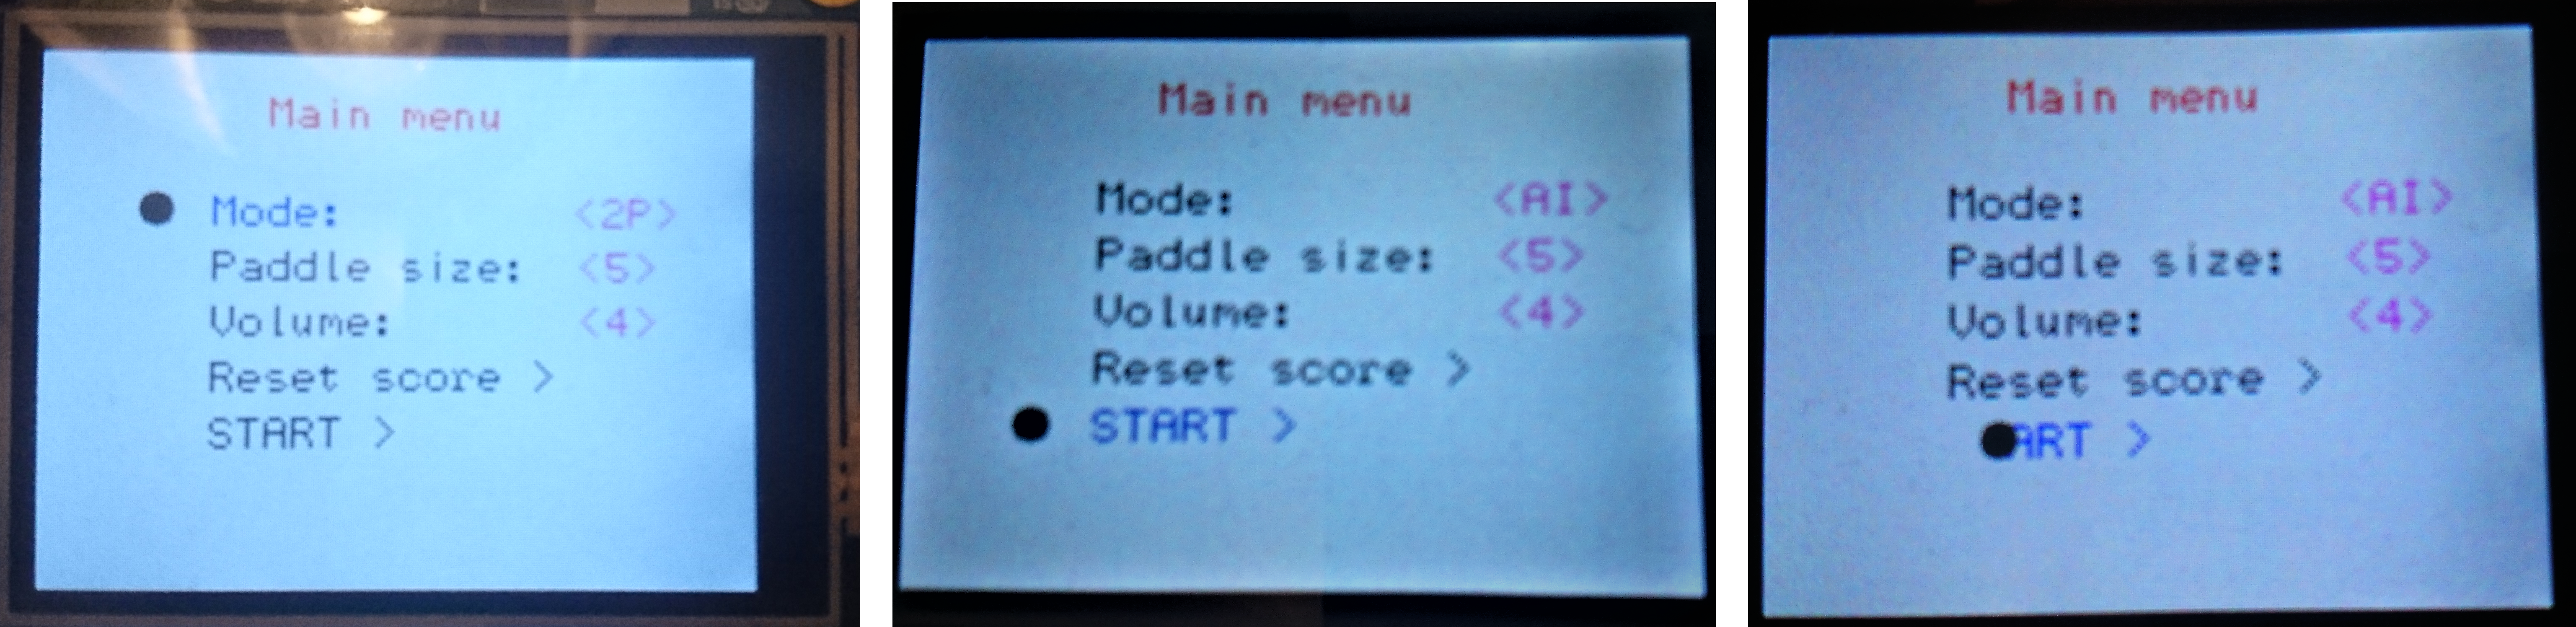
\includegraphics[width=0.9\textwidth]{./images/Menus_Combined.jpg}}
	\caption{Menus, showing choice of item, option, and the animation which runs on START}
\end{figure}
\- \\
The first option, Mode, dictates the game mode, and works simply by changing the \textit{gameMode} variable which is passed to 'setInputMode' on starting a game. Second is the paddle size, which changes the paddle size with 'pongSprites\_changePaddleSize'. This function was built especially, and works on the formula $Length_y (px) = 60+(size - 5)\times10$ - hence the default option of 5 (out of 10) gives a paddle height of 60 pixels.
\\ \- \\  
The volume setting was slightly more difficult, as it was decided that changing the volume should play a tone at the current amplitude defined by this setting. It was found that the blocking nature of sounds combined with the fact that 'menuMove' is called by interrupts caused the sounds to play forever; hence this option only changes the volume (using 'setVolume') and then the screen's main loop plays sounds if it sees a change in this setting.
\\ \- \\  
In order to reset the score, a function was added to pongEngine, which simply sets the scores for each player to zero. Finally, the start button resets the score if \textit{gameMode} has changed, and then sets the input mode, allowing the menu loop to end and return to main(). An animation runs on pressing START, which moves the ball across the start text, erasing it.
\\ \- \\  
It was initially found that if inputs were pressed whilst the menu items were changing, a bug occurred where the display did not accurately depict the current menu items selected. This was remedied by disabling the inputs and re-enabling either side of 'menuMove', using 'enableInputs'.
\end{flushleft}



\newpage
\section{Audio Output}
\begin{flushleft}
This section explains the method used to implement sounds in the final design. In order to include sounds, the DE1-SoC WM8731 and I2C drivers were utilised in combination with an example code. \textit{[Reference T. Carpenter’s work from lab 4??]}. It was noted initially that the code was slow to perform due to the float arithmetic involved in calculating the sinusoid of an angle, which caused the FIFO buffer of the audio device to overflow. We realised therefore that there were 2 real ways of approaching the problem: either, to utilise the onboard FPU of the DE1-SoC, or to create a faster approximation of the $\sin\theta$ function.
\\ \- \\
The code below demonstrates the fast sin function that was devised. The values of $\sin\theta$ from $0\degree$ to $90\degree$ were first calculated in Matlab, multiplied by $10^5$ and rounded to whole numbers. These results were then copied into a lookup table within the ‘lookupSin(unsigned int degree)’ macro. The storing of the numbers as fixed integers as opposed to floating point numbers served to save on memory usage.

\begin{figure}[H]
	\centering
	\lstinputlisting[language=C, firstline=1, lastline=16, frame=bt]{./Report_Code/fakePongSound.c}
	\caption{Code used produce fast sin lookup results for whole degrees.}
\end{figure}

\- \\
By utilising the characteristics of the $y=\sin\theta$ function over the period $0\degree$ to $180\degree$, where [y] is mirrored about $x=90\degree$, and the characteristic that the function is mirrored about $y=0$ at $x=180\degree$, it was then possible to find an approximation of $\sin\theta$ for any whole positive integer $\theta$ up to $360\degree$. Within the Sound macro, the float input to ‘lookupSin’, indicating the phase, was wrapped to a maximum of 360\degree and cast to an integer type. The maximum error in this lookup function at whole integers was approximately $4.9\times10^{-6}$.
\\ \- \\
The 'Sound(int \_freq, float \_duration)' macro first checks if sounds are flagged as on (via the \textit{SoundOn} variable). If so, a timer ISR is created to run for the period length. The phase is then incremented by a set amount determined by the frequency argument. The sounds are pushed to the WM8731 FIFOs and played in a while loop which checks the \textit{sound} variable. When the timer ISR triggers, \textit{sound} is changed to 0 and the Sound function finishes. It was initially noted that during gameplay, key presses caused gaps in sounds, so the 'Sound' macro temporarily disables inputs for the duration it runs.
Variable volume was implemented by adding a \textit{VOLUME} variable, which can be changed globally using the 'setVolume(int \_volume)' macro. The amplitude sent to the WM8731 is set as $2^{23+VOLUME}$, by bitshifting the value $2^{23}$ left VOLUME bits.
In order to make sound generation more intuitive, an additional header file was created containing the frequencies of musical notes from A3 to G6, and then sound macros were created for the various components of the game, including paddle collisions, scoring, and the start sound.
\end{flushleft}

\newpage
\section{Game Physics}
\begin{flushleft}
This section of the report details the physics engine of the game which is used to regulate the movement of the ball and its interactions with the paddles and the arena borders. 
\end{flushleft}
\subsection{Collisions}
\begin{flushleft}
Collisions are very important in a game of Pong as they are the only means by which the player can interact with the ball. The code in this project has been designed so that the ball moves through the game arena with a speed and angle that can be changed by collisions with the border and the paddles. Each paddle is divided into sectors which each produce different outgoing speed and angle values. Sectors that produce a more pronounced outcome, and therefore one more likely to surprise the other player, are smaller and more difficult to hit. A skilful player should be able to anticipate the path of the ball and align their paddle accordingly to gain maximum advantage from the collision. 
\\ \- \\
Figure 15 shows a schematic of the paddle with its collision sectors. Shown in yellow is sector 1, where the ball is perfectly reflected (i.e. angle of reflection = angle of incidence) and the outgoing speed is lowest. This sector is the largest as it gives the least amount of advantage to the player; the rebound angle is predictable and the outgoing speed is relatively easy to manage. Sector 2 is the second largest sector as it gives a 10 degree angle change and a medium outgoing speed. Sector 3 is the smallest and gives the largest change in angle with 20 degrees and the highest outgoing speed. 
\\ \- \\
\begin{figure}[H]
  \centering
  \fbox{\includegraphics[width=0.1\textwidth]{./images/JohnFigs/1.png}}
  \caption{showing location and relative size of each sector on the paddle.}
\end{figure}
\newpage
\subsection{Code Architecture}
The code for the physics of the game engine has its origin in the pongScreens.c file. This is where the game actually runs from and contains the while loop in which the ball is moved, and hence also where the collision checks occur. Six sets of collision checks are included within this while loop; two for the paddle collisions, two for each of the horizontal border collisions and two for the vertical sides of the arena. This latter set is not involved in the game physics as when a collision occurs here the game is reset and a point is added to the opposing player. 
\\ \- \\
The code for the horizontal border collisions is quite simple. Within the while loop in pongScreens, the collision check for the horizontal sides of the arena is triggered when the ball enters a predefined space, defined as 20 pixels from the top of the screen or 10 pixels from the bottom. When the ball enters this area, a new angle is retrieved from the function pongPhysics\_borderCollision with the new angle simply calculated as the negative of the incoming angle. For example, an incoming angle of 20 degrees will produce an outgoing angle of negative 20 degrees to the horizontal (left being 0) as shown in figure 16.
\begin{figure}[H]
  \centering
  \fbox{\includegraphics[width=0.4\textwidth]{./images/JohnFigs/2.png}}
  \caption{showing 20 degree collision with border and subsequent rebound}
\end{figure}
\- \\
The code for the paddle collisions is more complicated than that for border collision although it is similar. In much the same way, the check for the border collision takes place in the while loop within pongScreens. Defined as 15 pixels in front of the paddle (whose length can be varied), when a collision check occurs, a new value for the speed and the angle is obtained from pongPhysics\_borderCollision and used to move the ball until a new collision is made. This is done by subtracting the incoming angle from 180 degrees and adding to it a value called deltaAngle. deltaAngle is determined by the point on the paddle with which the ball collides, and is either 0, 10 or 35 (or their negative equivalent) depending on the sector with which the ball collides. A section of code is then used to make sure the angle stays within a constant frame of reference. In much the same way, a new velocity is calculated depending on what sector the ball collides with the velocities from sectors 2 and 3 being increasingly large. The inbound speed has no bearing on the calculated outbound speed. The angle and outbound speed are instantiated as a pointer-array and returned to pongScreens. The array is then read there and the new velocity and angle used to move the ball.
\newpage
Two flowcharts of the code that regulates the collisions are shown below :
\begin{figure}[H]
    \centering
    \subfloat[Flowchart for new angle/speed calculation]{{\includegraphics[width=7cm]{./images/JohnFigs/3.png} }}%
    \qquad
    \subfloat[Flowchart for collision checks]{{\includegraphics[width=7cm]{./images/JohnFigs/4.png} }}%
    \caption{flowcharts of the code that regulates the collisions}%
    \label{fig:example}%
\end{figure}

\section{AI}
The AI is extremely basic, and works by comparing the P2 paddle Y location and the ball Y location. At each iteration of the game's while loop, the paddle moves in the direction of the ball. It was found initially that this caused the paddle to jerk, as the paddle was making movements larger than the ball was; this was remedied by adding an extra region about the paddle's centre in the Y direction, hence it only moves when the ball is more than 10 px above or below from the centre of the paddle.

\end{flushleft}
\newpage
\section{Problems Encountered}
\begin{flushleft}
This sections details some of the many bugs that were encountered in the creation of the physics engine and the solutions that were employed in fixing them.
\end{flushleft}
\subsection{Ball becoming stuck at border/ paddle}
\begin{flushleft}
This was one of the earliest bugs encountered in the creation of the physics engine. When the ball collided with the paddle or the game border, it would become stuck, breaking the game and requiring a reset. This was caused by the direction (angle) of the ball constantly changing to the new value and then resetting to the new value as the ball remained within the collision space. This was fixed by introducing the pongEngine\_moveBall command into the pongPhysics\_borderCollision function. This ‘kicks’ the ball out of the collision space before allowing the pongEngine\_moveBall function within the while loop to continue moving the ball afterwards.
\end{flushleft}
\subsection{Ball moving through paddle at collision}
\begin{flushleft}
This bug has arisen several times throughout the development of the physics engine. Simply put, the ball is not affected by the collision boundaries at the paddle wall and instead travels straight through the paddle. Its difficult to predict when this happen and therefore difficult to step through the code and test for it, however it seems to only happen infrequently as of the latest build. Eariler versions of the bug seem to have been caused by the new angle calculations being incorrect as the calculated value exceeded 360. Introducing code that keeps the angle calculations within a constant frame of reference (ie between 0 and 180/-180) seems to have drastically reduced its frequency, although it can still happen on occasion.
\end{flushleft}
\subsection{Ball disappearing after paddle collision}
\begin{flushleft}
his bug was particularly difficult to resolve even though the fix was ultimately quite simple. When the ball collided with a paddle wall it would sometimes randomly disappear without forewarning. Again, this was quite difficult to test for due to the unpredictable nature of the bug. Using breakpoints in the code eventually uncovered the problem. Sometimes when a paddle collision was made, the ball would collide with a part of the paddle not covered by the series of if-else statements in the pongPhysics\_paddleCollision code. As such, no value was assigned to the variable ‘outspeed’ when it was returned to the pongScreens file. A nonsensical random value, usually quite large, was instead assigned, causing the ball to have an impossibly high speed and disappear from view. This was fixed by initialising the ‘outspeed’ variable with 0, and introducing an ‘else’ statement that would cover what to do in such a situation.
\end{flushleft}
\newpage
\section{Conclusion}
\begin{flushleft}
To conclude, a version of the well known game Pong was programmed using the DE1-SoC Development Board from Terasic. Code was written in C and compiled and debugged using the ARM DS-5 suite of software. The design incorporated the use of a range of hardware peripherals and outputs including VGA, LCD, PS/2, audio jack and 7-segment display. The game has been designed to be played either single player against a simple AI or against another player. A menu system has been created allowing the player to select the mode they wish to play in as well as the size of the paddles in the game. The coding architecture and general approach to the project have been described as have the bugs/problems encountered during the course of the project. 
\\ \- \\
The code for the game was extensively tested and debugged through hardware testing. Generally the game is quite robust and functions well when subjected to testing. Nevertheless a few bugs still exist, particularly with regards to the ball’s behaviour when collisions occur within the game. Another bug would be screen tearing because of the multiple small frame buffers. Further testing and debugging should be conducted to address these issues. 
\end{flushleft}
\newpage
\section{Appendix \label{section:appendix}}
\subsection{Appendix A - sevenSeg.c}
\lstinputlisting[language=C, frame=bt]{../DE1_SOC_PONG/DE1SoC_SevenSeg/sevenSeg.c}
\newpage
\subsection{Appendix B - sevenSeg.h}
\lstinputlisting[language=C, frame=bt]{../DE1_SOC_PONG/DE1SoC_SevenSeg/sevenSeg.h}
\newpage
\subsection{Appendix C - DE1SoC VGA.c}
\lstinputlisting[language=C, frame=bt]{../DE1_SOC_PONG/DE1SoC_VGA/DE1SoC_VGA.c}
\newpage
\subsection{Appendix D - DE1SoC VGA.h}
\lstinputlisting[language=C, frame=bt]{../DE1_SOC_PONG/DE1SoC_VGA/DE1SoC_VGA.h}
\newpage
\subsection{Appendix E - pongDisplay.c}
\lstinputlisting[language=C, frame=bt]{../DE1_SOC_PONG/pongDisplay/pongDisplay.c}
\newpage
\subsection{Appendix F - pongDisplay.h}
\lstinputlisting[language=C, frame=bt]{../DE1_SOC_PONG/pongDisplay/pongDisplay.h}
\newpage
\subsection{Appendix G - pongEngine.c}
\lstinputlisting[language=C, frame=bt]{../DE1_SOC_PONG/pongEngine/pongEngine.c}
\newpage
\subsection{Appendix H - pongEngine.h}
\lstinputlisting[language=C, frame=bt]{../DE1_SOC_PONG/pongEngine/pongEngine.h}
\newpage
\subsection{Appendix I - pongSprites.c}
\lstinputlisting[language=C, frame=bt]{../DE1_SOC_PONG/pongEngine/pongSprites.c}
\newpage
\subsection{Appendix J - pongSprites.h}
\lstinputlisting[language=C, frame=bt]{../DE1_SOC_PONG/pongEngine/pongSprites.h}
\newpage
\subsection{Appendix K - pongPhysics.c}
\lstinputlisting[language=C, frame=bt]{../DE1_SOC_PONG/pongEngine/pongPhysics.c}
\newpage
\subsection{Appendix L - pongPhysics.h}
\lstinputlisting[language=C, frame=bt]{../DE1_SOC_PONG/pongEngine/pongPhysics.h}
\newpage
\subsection{Appendix M - pongInputs.c}
\lstinputlisting[language=C, frame=bt]{../DE1_SOC_PONG/pongInputs/pongInputs.c}
\newpage
\subsection{Appendix N - pongInputs.h}
\lstinputlisting[language=C, frame=bt]{../DE1_SOC_PONG/pongInputs/pongInputs.h}
\newpage
\subsection{Appendix O - pongSounds.c}
\lstinputlisting[language=C, frame=bt]{../DE1_SOC_PONG/pongSound/pongSound.c}
\newpage
\subsection{Appendix P - pongSounds.h}
\lstinputlisting[language=C, frame=bt]{../DE1_SOC_PONG/pongSound/pongSound.h}
\newpage
\subsection{Appendix Q - pongScreens.c}
\lstinputlisting[language=C, frame=bt]{../DE1_SOC_PONG/pongScreens/pongScreens.c}
\newpage
\subsection{Appendix R - pongScreens.h}
\lstinputlisting[language=C, frame=bt]{../DE1_SOC_PONG/pongScreens/pongScreens.h}
\newpage
\subsection{Appendix S - main.c}
\lstinputlisting[language=C, frame=bt]{../DE1_SOC_PONG/main.c}
\newpage
\addcontentsline{toc}{section}{References}
\begin{flushleft}
\bibliography{refs}
\end{flushleft}
\end{document}
